\chapter{A Wider View: Models of Other Supernova Remnants}\label{chp:chp6}

%\begin{flushright}
%  {\em QUOTE GOES HERE }\\
%
%\ \
%
%\normalsize
%{AUTHOR}  
%\end{flushright}


\noindent{FIRST PARAGRAPH}

\section{Introduction}
\section{SN~1980K}
\section{SN~1993J}
\section{Cassiopeia A}

\section{Models of Late-Time Line Profiles from Core-Collapse Supernovae}

\subsection{Smooth Models}
\begin{figure}
\centering
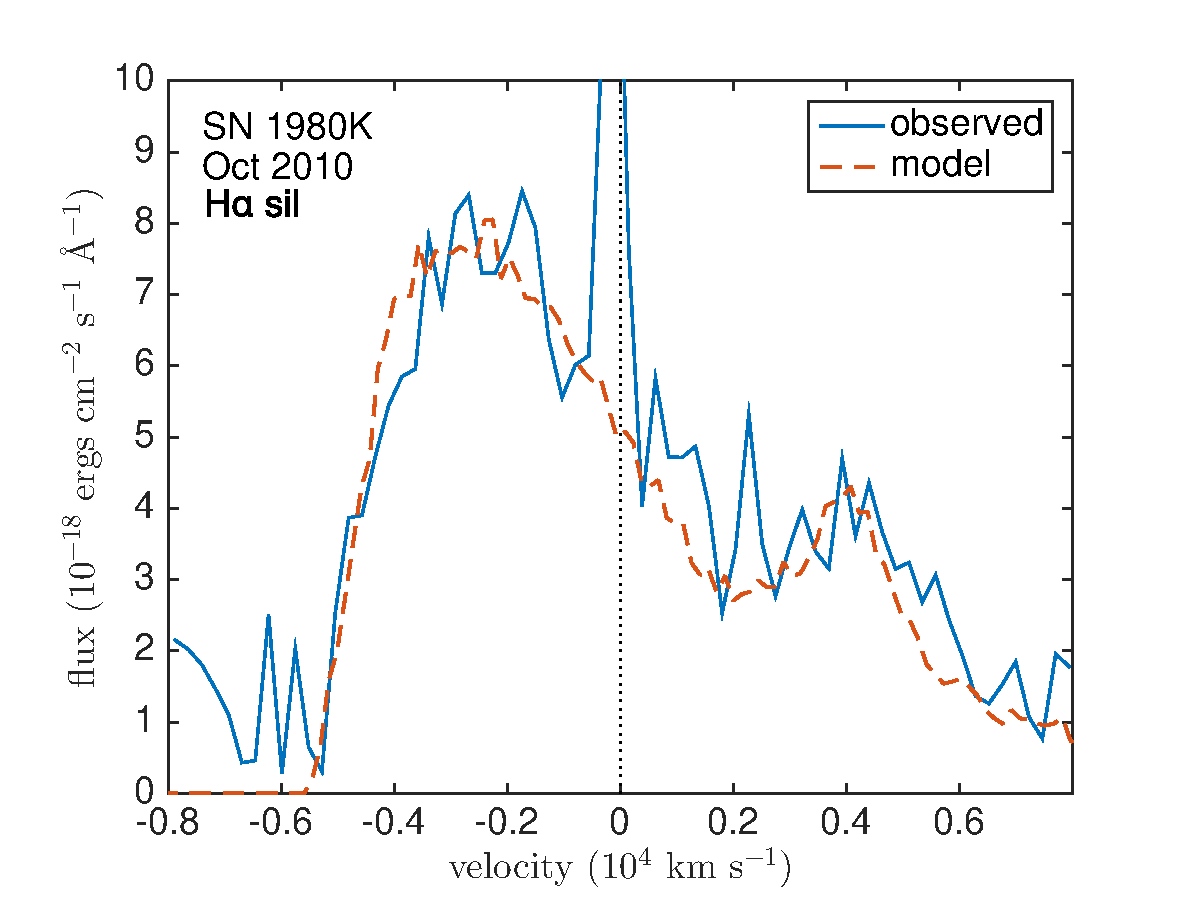
\includegraphics[scale=0.4,clip=true, trim=20 0 40 20]{chapters/chapter6/figs/80K/smooth/Ha}
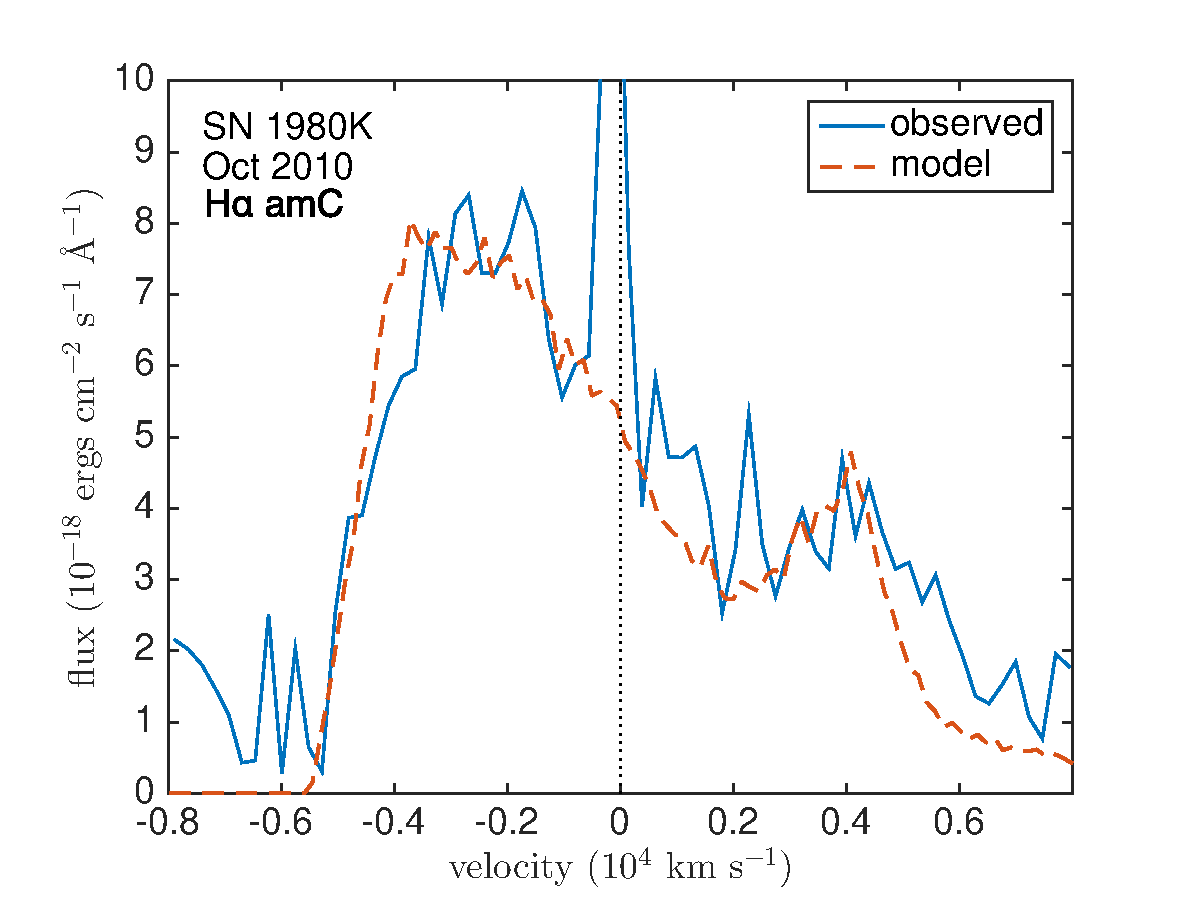
\includegraphics[scale=0.4,clip=true, trim=20 0 40 20]{chapters/chapter6/figs/80K/smooth/Ha_amC}

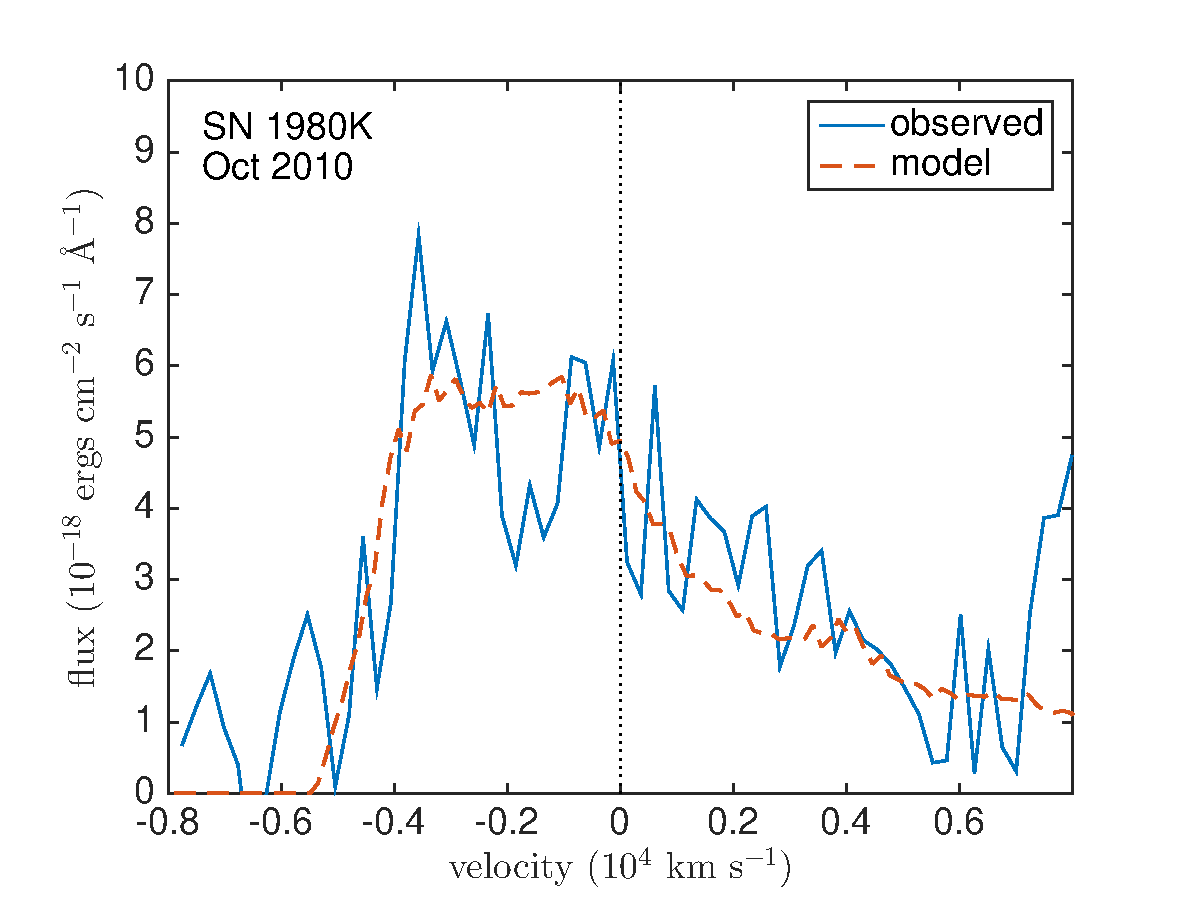
\includegraphics[scale=0.4,clip=true, trim=20 0 40 20]{chapters/chapter6/figs/80K/smooth/OI}
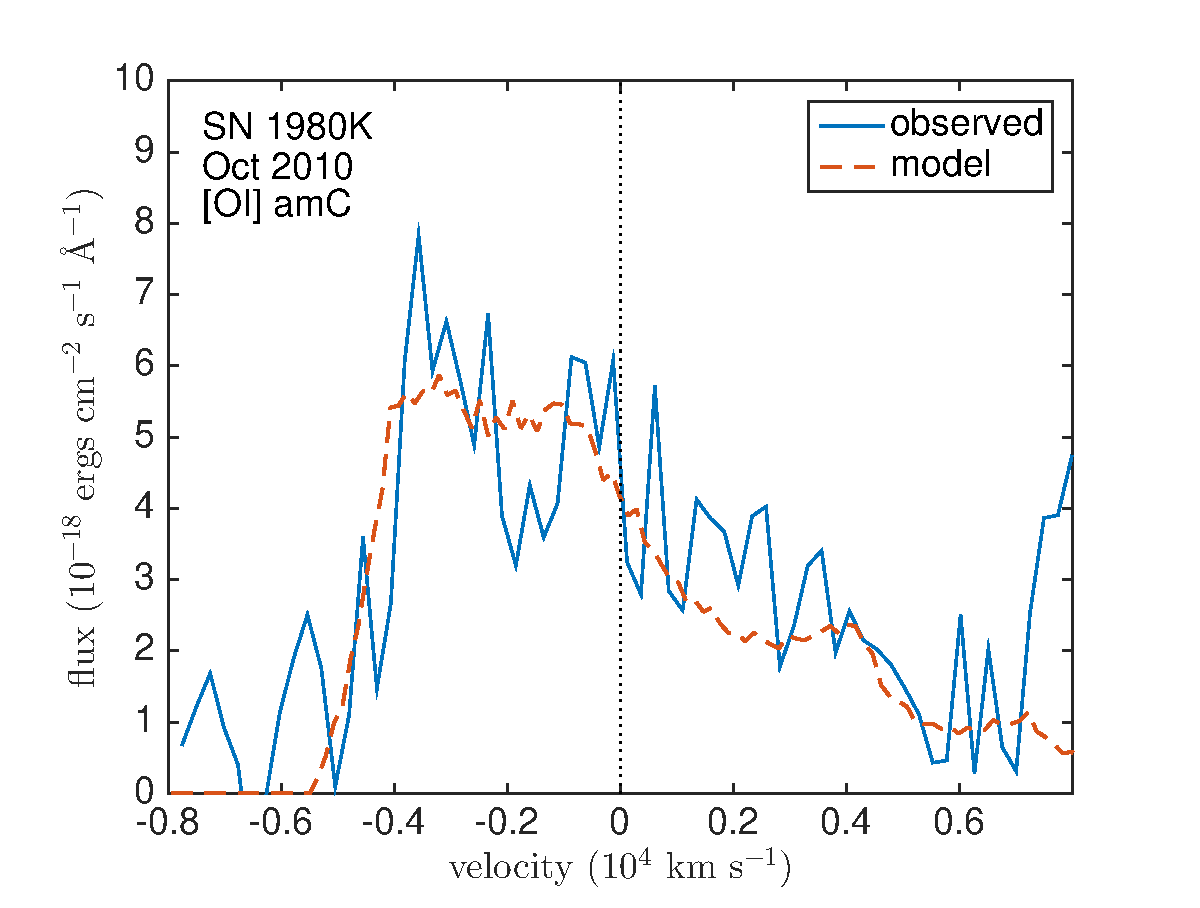
\includegraphics[scale=0.4,clip=true, trim=20 0 40 20]{chapters/chapter6/figs/80K/smooth/OI_amC}
\caption{Smooth fits to SN 1980K}
\label{80K_smooth}
\end{figure}

\begin{figure}
\centering
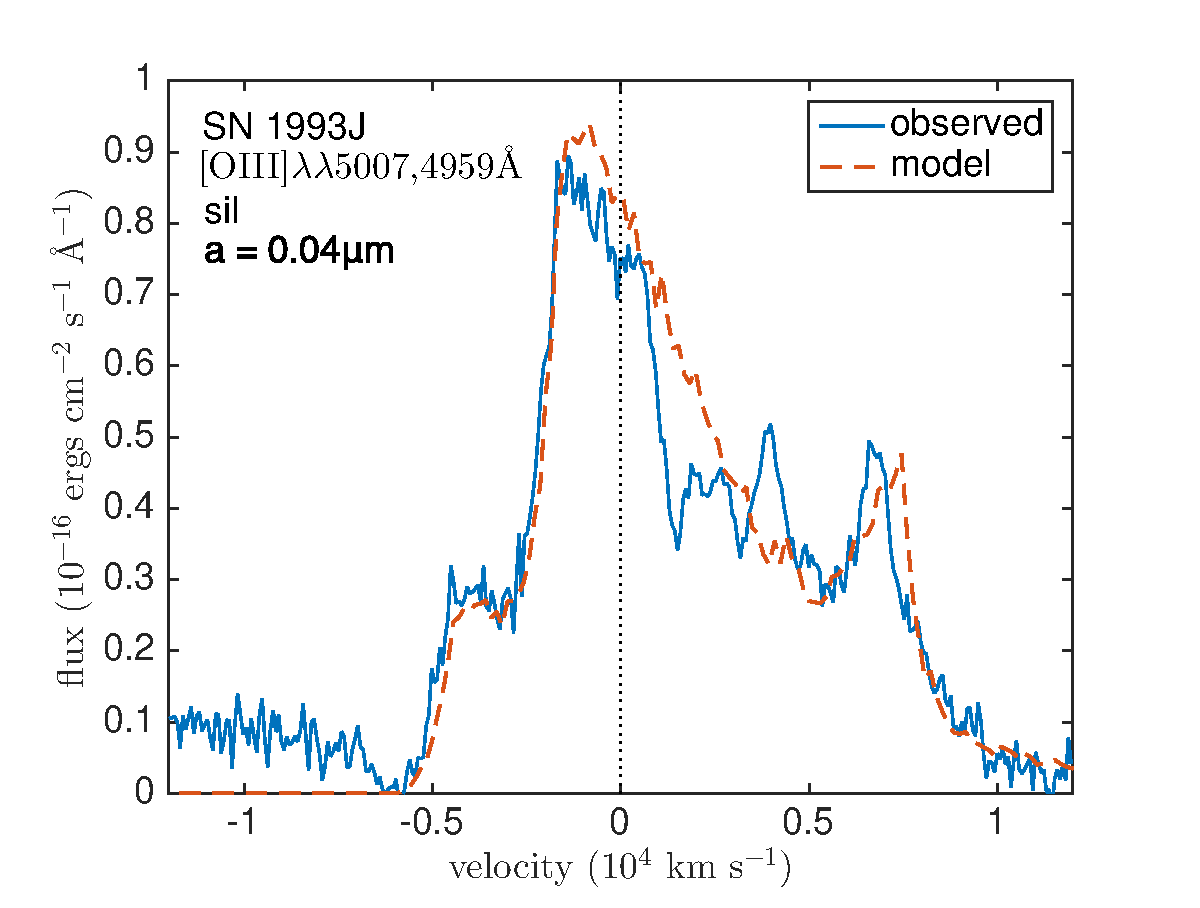
\includegraphics[scale=0.4,clip=true, trim=20 0 40 20]{chapters/chapter6/figs/93J/smooth/OIII}
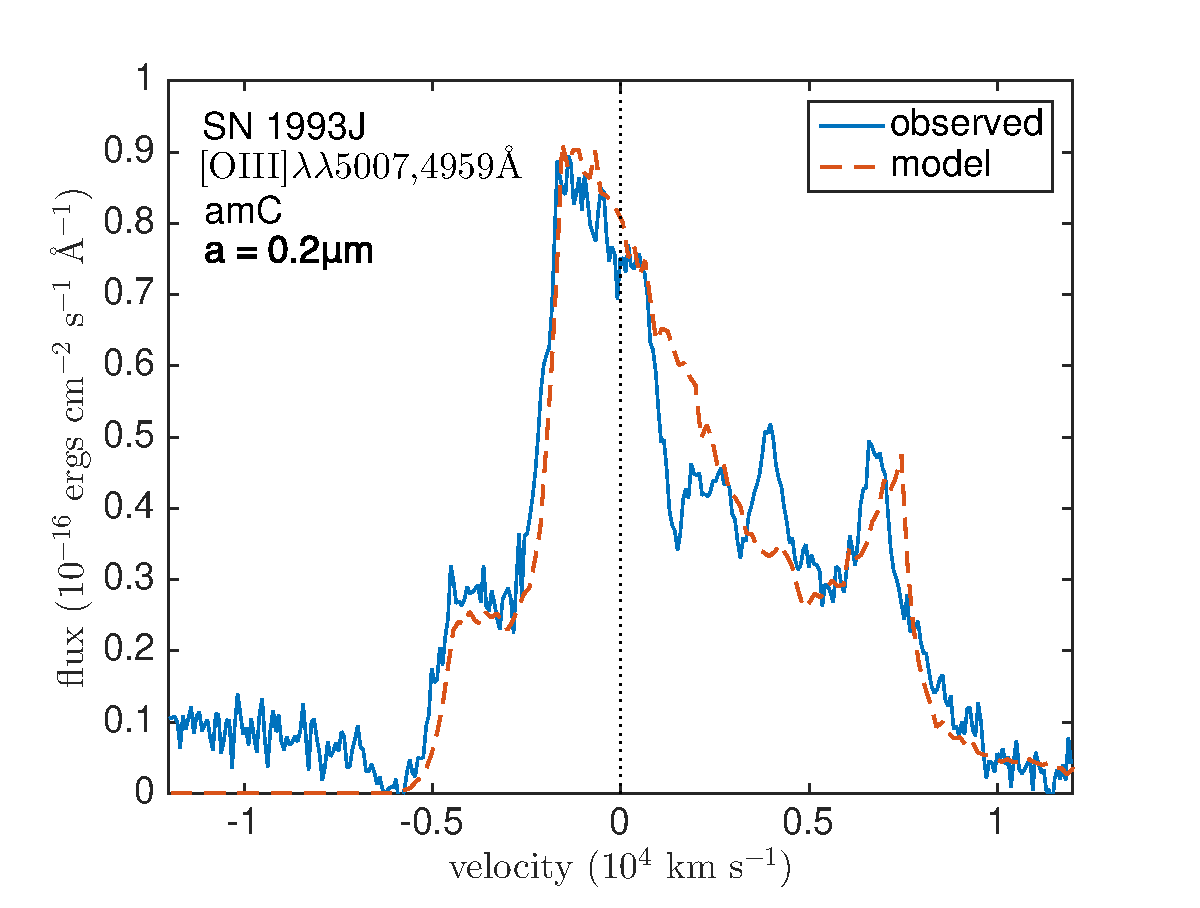
\includegraphics[scale=0.4,clip=true, trim=20 0 40 20]{chapters/chapter6/figs/93J/smooth/OIII_amC}

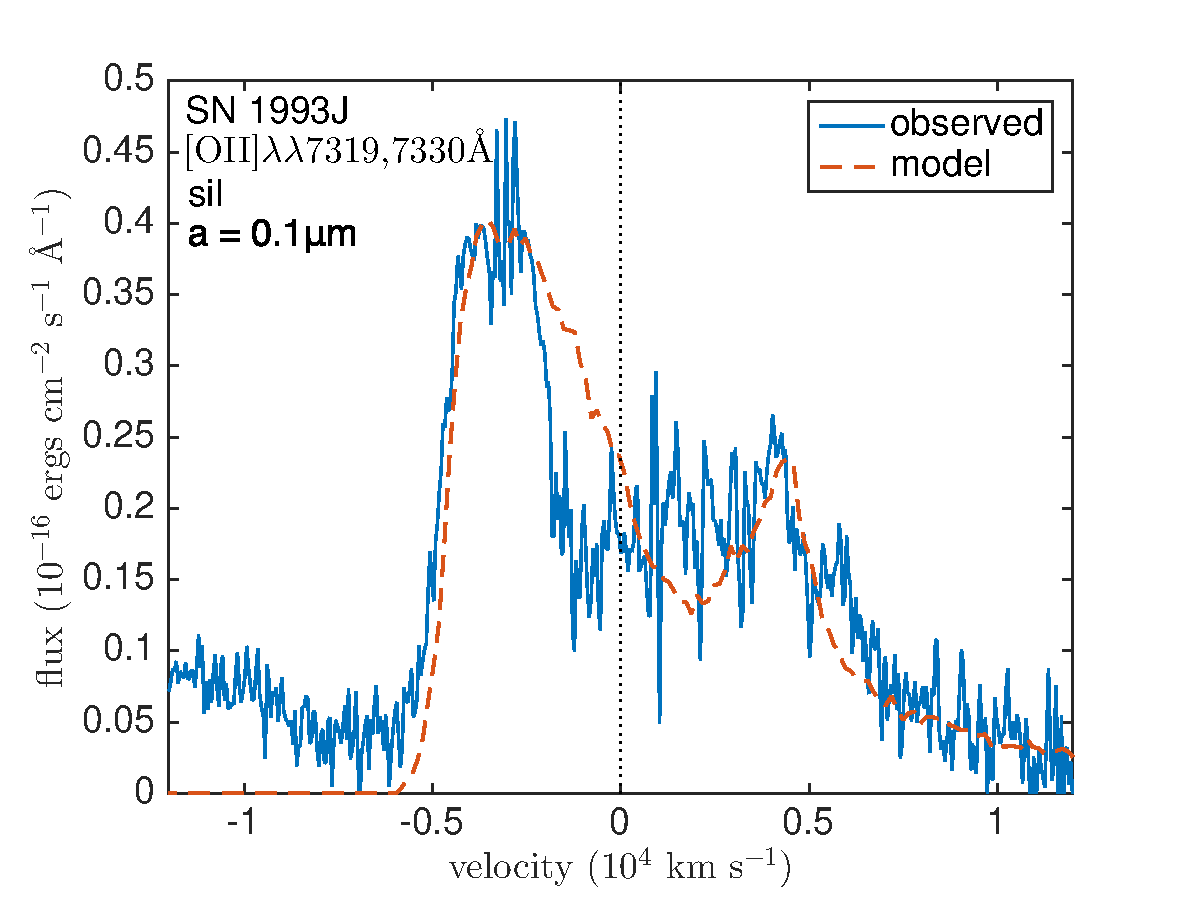
\includegraphics[scale=0.4,clip=true, trim=20 0 40 20]{chapters/chapter6/figs/93J/smooth/OII}
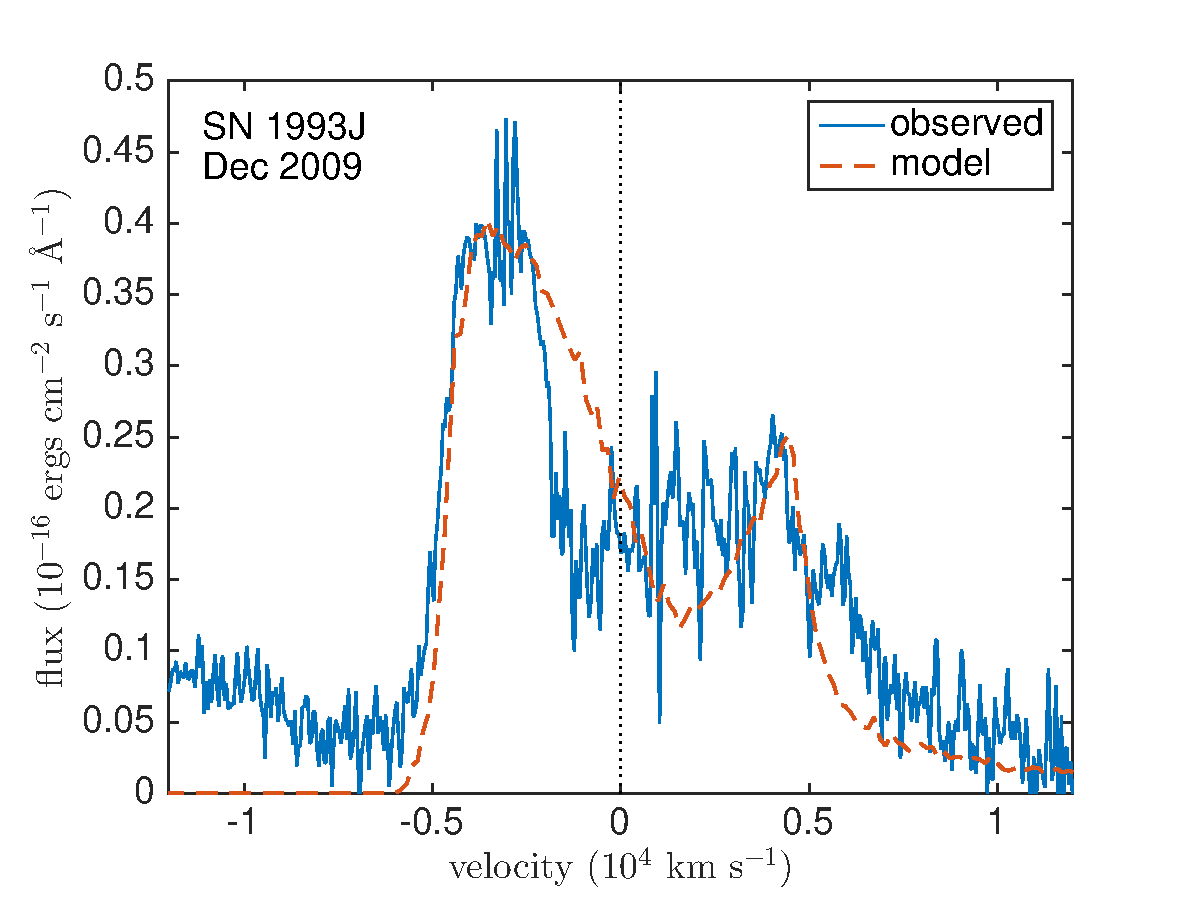
\includegraphics[scale=0.4,clip=true, trim=20 0 40 20]{chapters/chapter6/figs/93J/smooth/OII_amC}
\caption{smooth fits to SN 1993J}
\label{93J_smooth}
\end{figure}

\begin{figure}
\centering
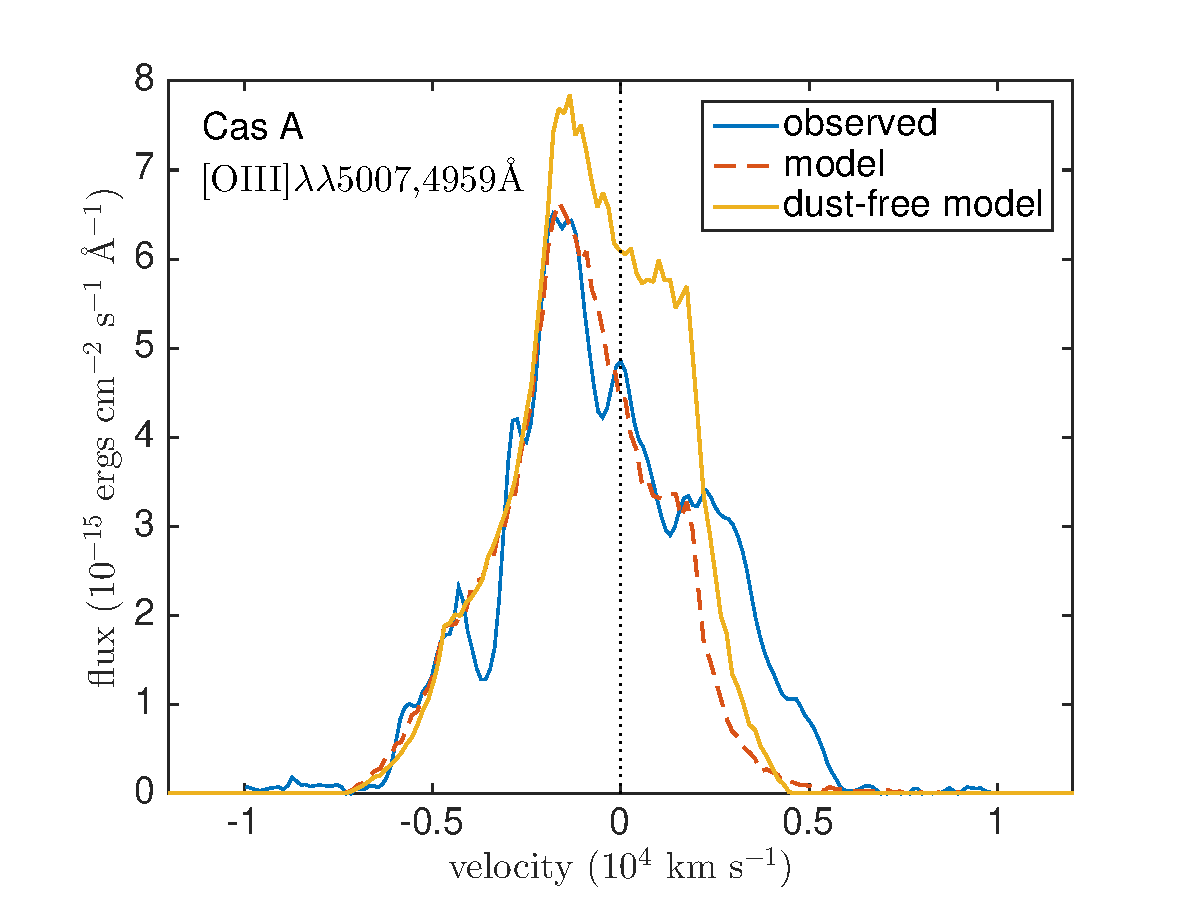
\includegraphics[scale=0.4,clip=true, trim=20 0 40 20]{chapters/chapter6/figs/CasA/CasA_OIII}
\caption{smooth fits to Cas A}
\label{CasA}
\end{figure}

\subsection{Clumped Models}

\begin{figure}
\centering
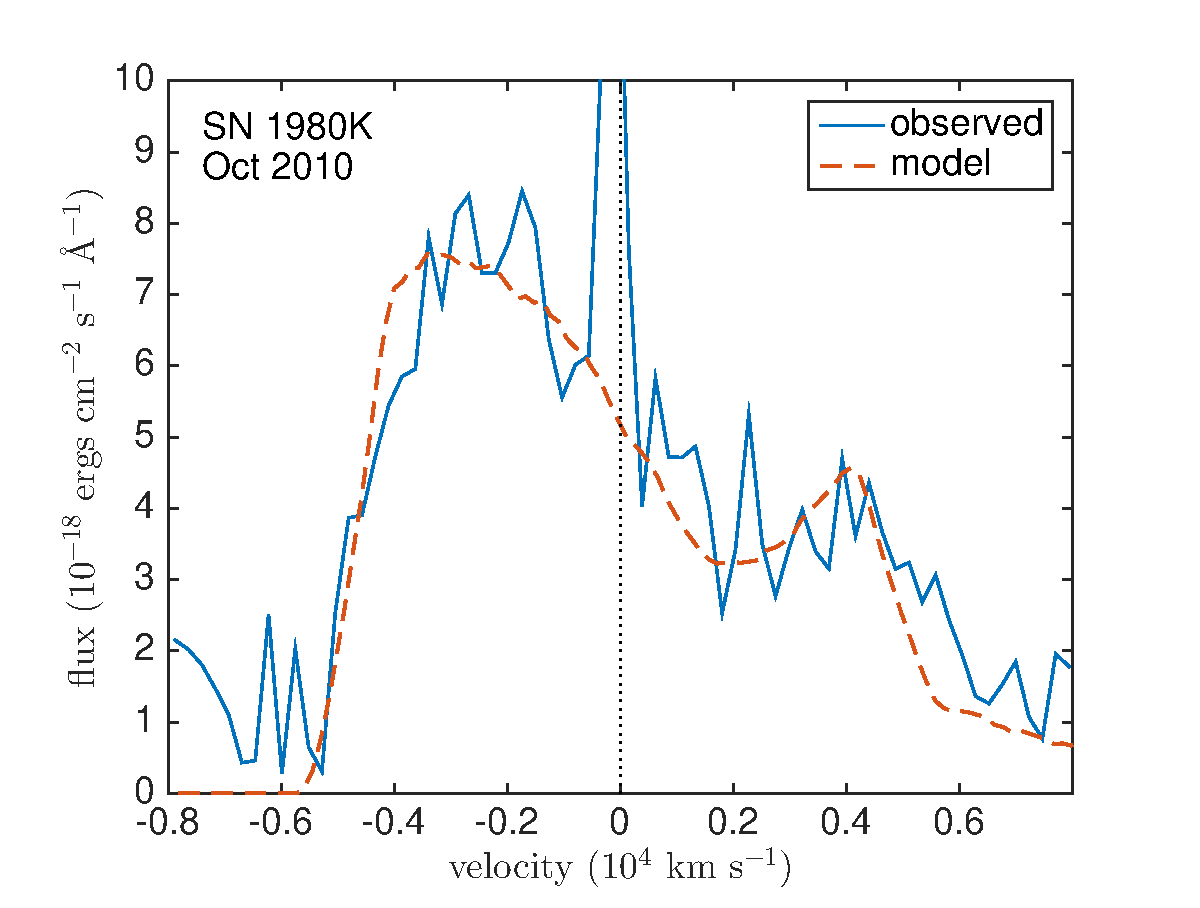
\includegraphics[scale=0.4,clip=true, trim=20 0 40 20]{chapters/chapter6/figs/80K/clumped/Ha}
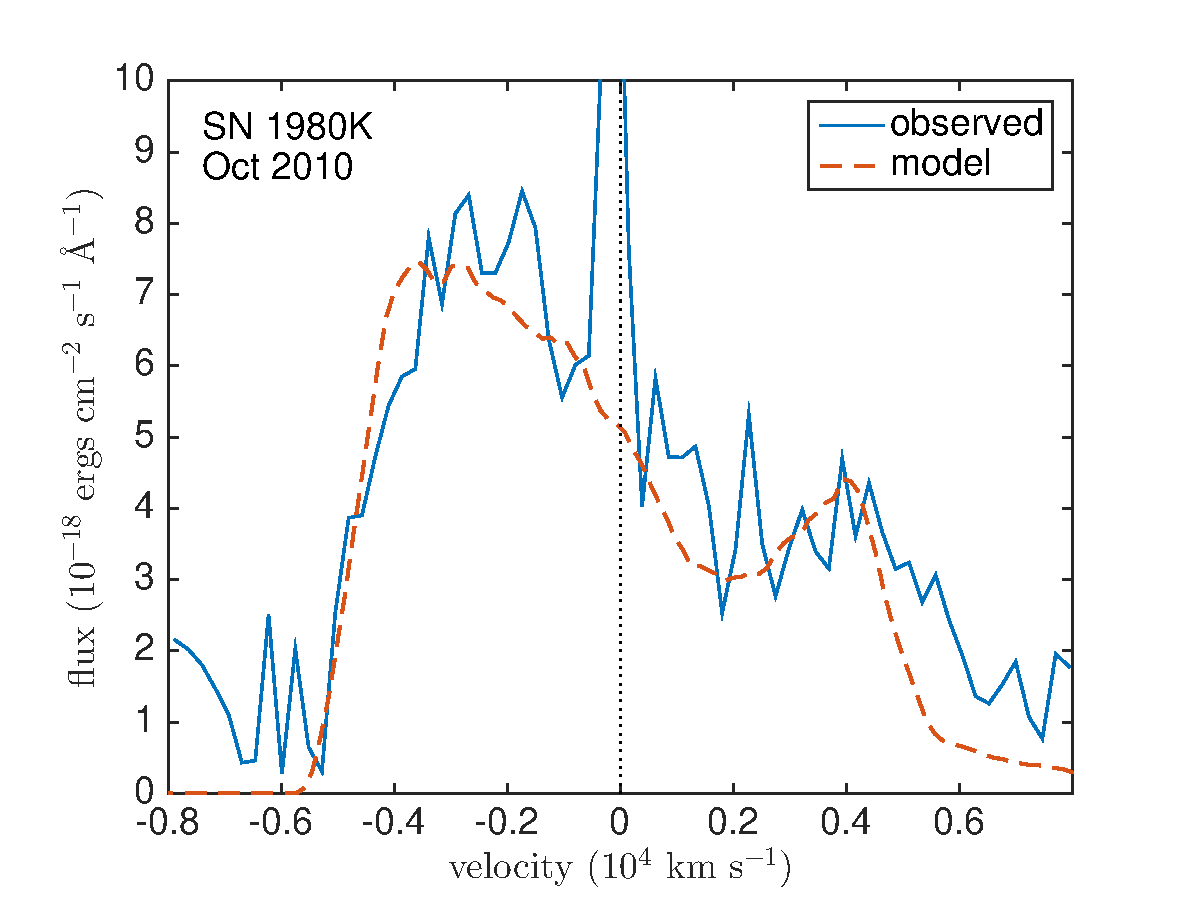
\includegraphics[scale=0.4,clip=true, trim=20 0 40 20]{chapters/chapter6/figs/80K/clumped/Ha_amC}

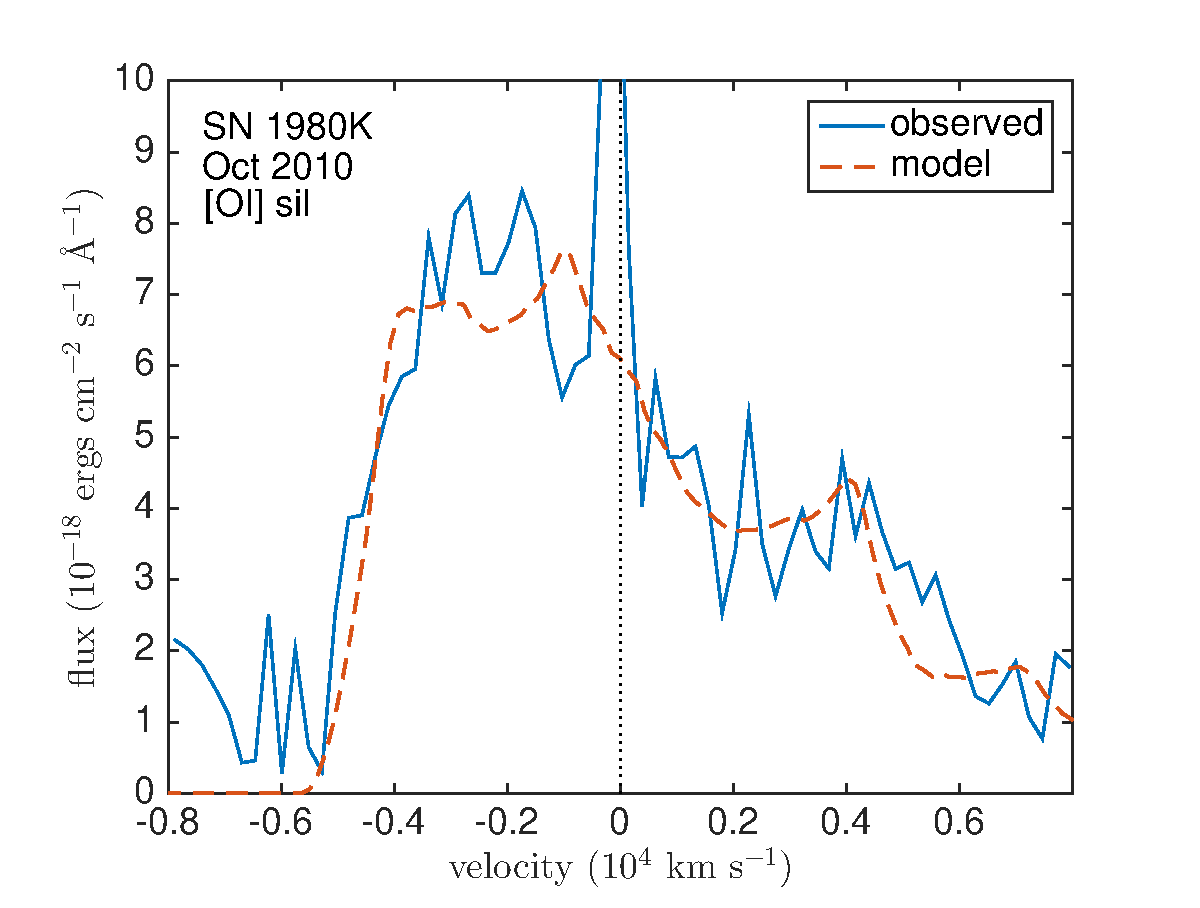
\includegraphics[scale=0.4,clip=true, trim=20 0 40 20]{chapters/chapter6/figs/80K/clumped/OI}
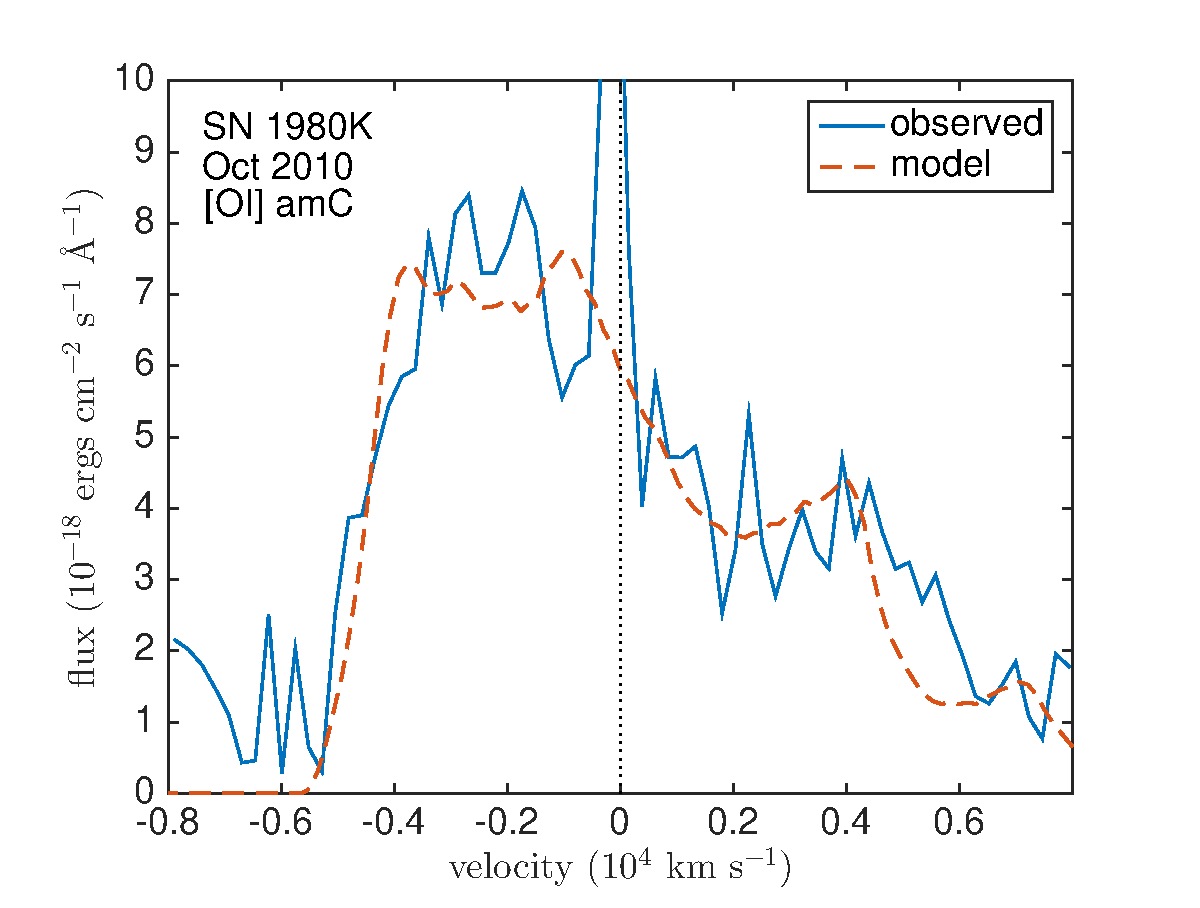
\includegraphics[scale=0.4,clip=true, trim=20 0 40 20]{chapters/chapter6/figs/80K/clumped/OI_amC}
\caption{clumped fits to SN 1980K}
\label{80K_clumped}
\end{figure}

\subsection{Velocity-Shifted Line Profile Models}

\begin{figure}
\centering
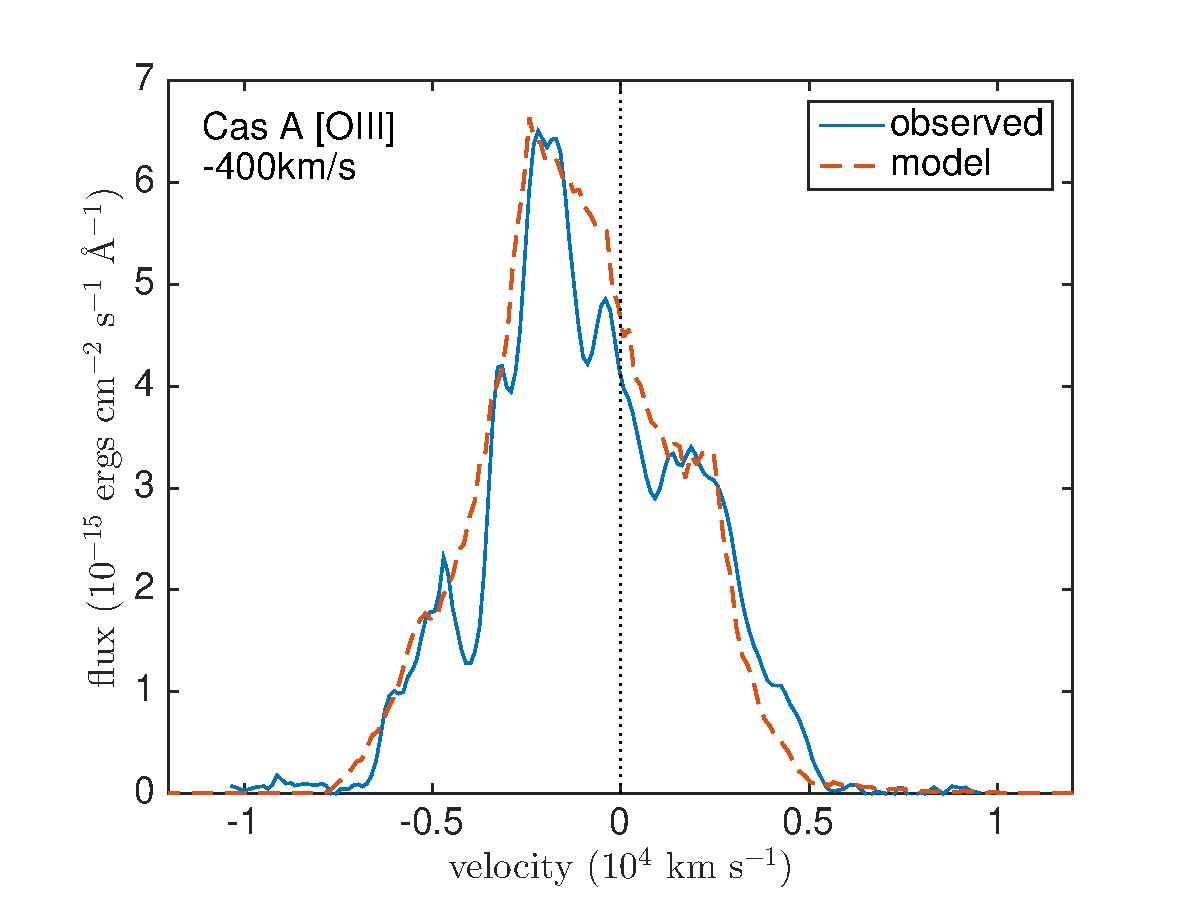
\includegraphics[scale=0.4,clip=true, trim=20 0 40 20]{chapters/chapter6/figs/CasA/CasA_OIII_v400shift}
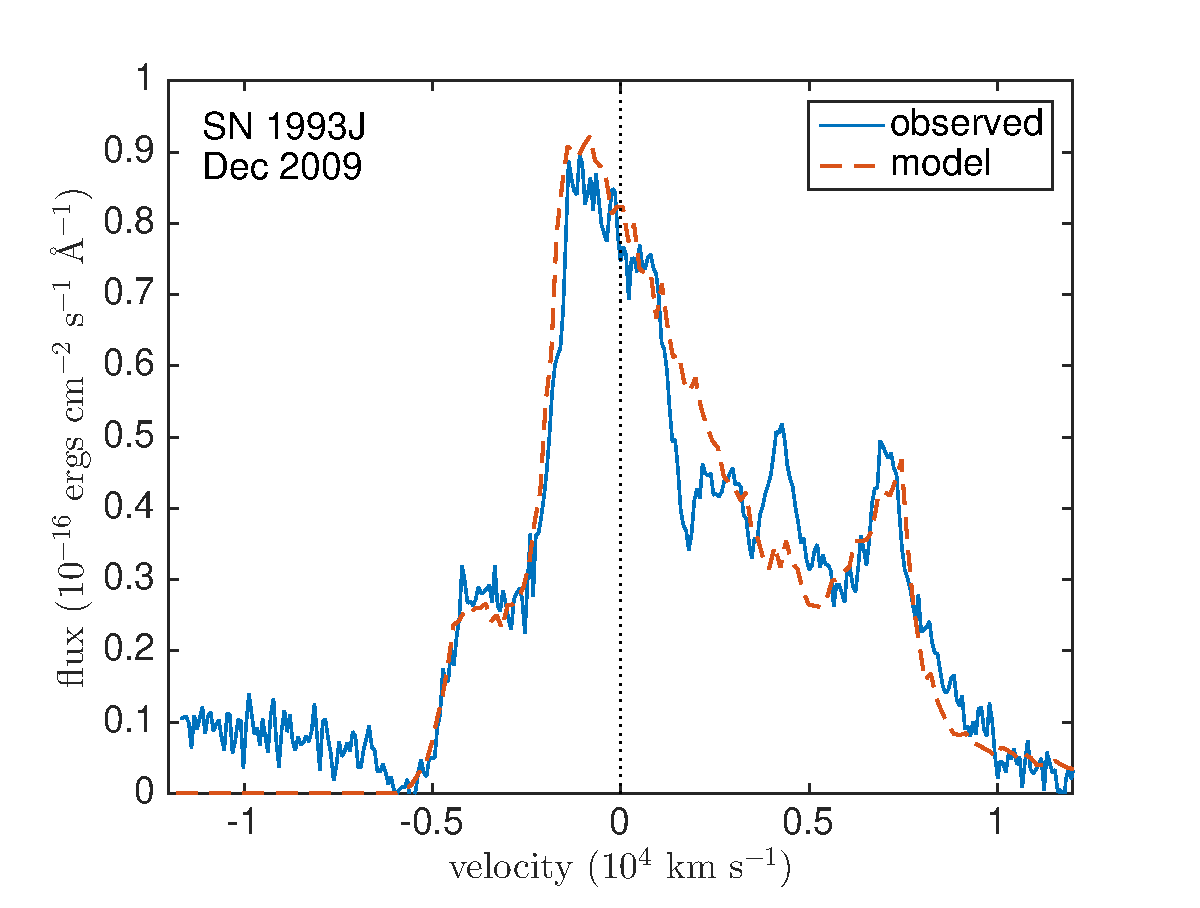
\includegraphics[scale=0.4,clip=true, trim=20 0 40 20]{chapters/chapter6/figs/93J/smooth/OIII_shifted_0_3}
\caption{shifted profiles of SN~1993J and Cas A}
\label{shifted}
\end{figure}


\section{Discussion}
\section{Conclusions}








